\documentclass[12pt,a4paper]{article}

% Margins.
\setlength{\oddsidemargin}{0in}
\setlength{\evensidemargin}{0in}
\setlength{\headheight}{12pt}
\setlength{\headsep}{42pt}
\setlength{\topmargin}{-54pt}
\setlength{\textwidth}{6.5in}
\setlength{\textheight}{10in}

\usepackage{amsmath}
\usepackage{float}
\usepackage{graphicx}
\usepackage[hyphens]{url}
\usepackage{hyperref}	% Clickable links to figures, references and urls.
\usepackage{datetime}
\usepackage{longtable}

% Drawing.
\usepackage{pgf}
\usepackage{tikz}

% Listings for formatting code.
\usepackage{listings}
\usepackage{textcomp}
% General options.
\lstset{breaklines=true, basicstyle=\small\ttfamily, tabsize=4, numbers=left, stepnumber=1, frame=single, showstringspaces=false, upquote=true}
% C++ specific high-lighting. Comments are 50/50 shades of green/black and strings coloured with 60/40 red/black mixture.
\lstset{language=[ISO]C++, commentstyle=\color{green!50!black}, keywordstyle=\color{blue}, stringstyle=\color{red!60!black}}

%opening
\title{\vspace{-2cm}Physics for Engineers\\Class 02\\Introduction to Scalars and Vectors}
\author{Attique Dawood}
\date{August 21, 2013\\[0.2cm] Last Modified: \today, \currenttime}
\begin{document}
\maketitle
Today's lecture is from sections 1.3--1.6 of reference book \cite{Sadiku}.
\section{Announcements}
\begin{itemize}
\item We're going to follow \cite{Sadiku} as reference book.
\item Text and reference books have been uploaded on SLATE.
\item We're not going to go into the details of one--dimensional kinematics. We will start with vector analysis today.
\end{itemize}
\section{Revision}
\begin{itemize}
\item The goal of this course is to understand Maxwell's equations that govern the working of electromagnetics.
\item Scientific and engineering notations.
\end{itemize}
\section{Scalars and Vectors (1.3S)}
\subsection{Scalars}
A scalar quantity has only magnitude. Distance, mass, time, etc. are examples of some scalars. A scalar quantity is represented by a plain letter, e.g, $A, t, m$.
\subsection{Vectors}
Vector quantities require a direction along with magnitude. If you want directions to the nearest restaurant and ask someone, you get an answer like this: ``Walk a distance of 100 m and you'll get there.'' Does this make any sense? You know how much distance you have to travel but you don't know which direction to go! Instead if you are told: ``Walk 100 m westward.'' This gives a complete description of where your destination is. Some examples of vectors are displacement, velocity, force, electric field, etc.

A vector quantity is represented by boldface (capital) letter or a letter with a bar or arrow above. Unit  vectors are usually represented with small boldface letters or with a hat above. Examples of vector notation are: $\textbf{{A}}, \vec{A}, \bar{A}, \textbf{x}, \hat{x}$.

Boldface notation is usually used in printed text. It is easier to use a bar for vectors in hand--written text.
\section{Unit Vector (1.4S)}
A vector \textbf{A} has both magnitude and direction. The \textit{magnitude} of vector \textbf{A} is a scalar quantity written as $A$ or $|\textbf{A}|$. A \textit{unit vector} $\hat{a}_A$ along \textbf{A} is defined as a vector that has the same direction as \textbf{A} but a magnitude of 1.
\begin{equation}
\hat{a}_A=\dfrac{\textbf{A}}{|\textbf{A}|}=\dfrac{\textbf{A}}{A}
\end{equation}
Note that $|\hat{a}_A|=1$. Vector \textbf{A} can be written as,
\begin{equation}
\textbf{A}=A\hat{a}_A
\end{equation}
\section{Representation of Vectors in Cartesian Coordinate System}
A vector \textbf{A} in Cartesian coordinate system is written as,
\begin{equation}
(A_x,A_y,A_z)~or~\textbf{A}=A_x\hat{x}+A_y\hat{y}+A_z\hat{z}
\end{equation}
$A_x$, $A_y$ and $A_z$ are called \textit{components} of \textbf{A} in $x$, $y$ and $z$ directions, respectively. The unit vectors $\hat x$, $\hat y$ and $\hat z$ point in the increasing direction of $x$, $y$, and $z$.
\begin{figure}[H]
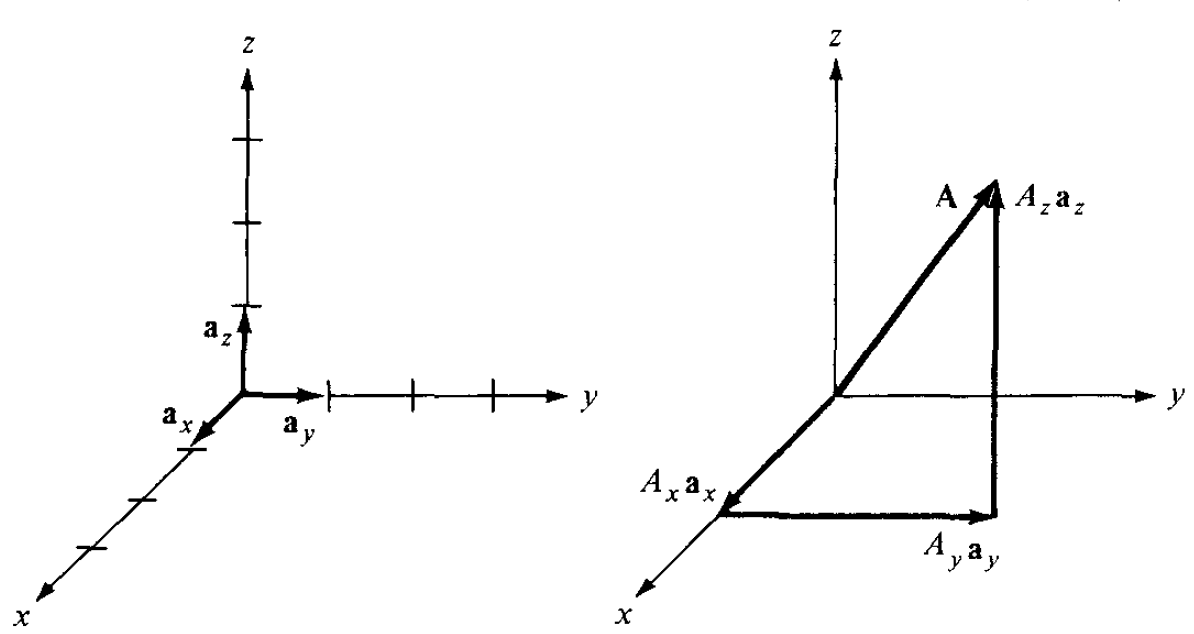
\includegraphics[scale=0.5]{Figure1-1S.png}
\caption{Representation of a vector in Cartesian coordinates \cite[fig. 1.1]{Sadiku}}
\label{components-of-A}
\end{figure}
The magnitude of \textbf{A} is given by,
\begin{equation}
|\textbf{A}|=A=\sqrt{A_x^2+A_y^2+A_z^2}
\end{equation}
The unit vector along \textbf{A} is given by,
\begin{equation}
\hat{a}_A=\dfrac{\textbf{A}}{A}=\dfrac{A_x\hat{x}+A_y\hat{y}+A_z\hat{z}}{\sqrt{A_x^2+A_y^2+A_z^2}}
\end{equation}
\section{Addition and Subtraction of Vectors (1.5S)}
Vectors \textbf{A} and \textbf{B} can be added together to give a third vector \textbf{C},
\begin{equation}
\textbf{C}=\textbf{A}+\textbf{B}
\end{equation}
If $\textbf{A}=(A_x,A_y,A_z)$ and $\textbf{B}=(B_x,B_y,B_z)$ then,
\begin{equation}
\textbf{C}=(A_x+B_x)\hat x+(A_y+B_y)\hat y+(A_z+B_z)\hat z
\end{equation}
Vector subtraction is carried out in a similar manner.
\begin{equation}
\textbf{D}=\textbf{A}-\textbf{B}=\textbf{A}+(-\textbf{B})=(A_x-B_x)\hat x+(A_y-B_y)\hat y+(A_z-B_z)\hat z
\end{equation}
Graphically, vectors are added or subtracted using the parallelogram rule or head--to--tail rule.
\section{Function}
\noindent\textbf{Warning:} This is a very loose definition of function but one that is convenient and suitable for us. In calculus you might come across a stricter definition.
\begin{itemize}
\item A function is a `rule' (or relationship) between two quantities.
\item Two variables, independent and dependent are associated with a function.
\item All possible values that independent variable can take is called `domain' of function.
\item All possible values that dependent variable can take is called `range' of function.
\item In the function $x(t)=2t$, $x$ is dependent variable, $t$ is independent variable and the rule is `value of $x$ is twice that of $t$' or simply $2t$.
\end{itemize}
\section{Scalar and Vector Fields}
\subsection{Field}
A field is a function of space or the coordinates x, y and z. A field specifies or defines a scalar quantity in the whole space or region.
\subsection{Scalar Field}
A scalar field is a function that assigns to each point in space a scalar or number. For example, temperature in a room at each point is defined by a function $T(x, y, z)=2x+3y-z$.
\subsection{Vector Field}
A vector field is a function that assigns to each point in space a vector. For example, electric field in a region is given by $\bar{E}(x, y, z)=2y\hat{x}+3z\hat{y}+xy\hat{z}$.
\section{Exercises}
\noindent\textbf{Question 1:} Given $\textbf{A}=10\hat x-4\hat y+6\hat z$ and $\textbf{B}=2\hat x+\hat y$, find,
\begin{enumerate}
\item[(1)] The scalar component of \textbf{A} along $\hat y$.
\item[(2)] The vector component of \textbf{A} along $\hat y$.
\item[(3)] The magnitude of $3\textbf{A}-4\textbf{B}$.
\item[(4)] A unit vector along $\textbf{A}+2\textbf{B}$
\end{enumerate}
\noindent\textbf{Question 2:} Given vectors $\textbf{A}=\hat x+3\hat z$ and $\textbf{B}=5\hat x+2\hat y-6\hat z$, find,
\begin{enumerate}
\item[(1)] $|\textbf{A}+\textbf{B}|$.
\item[(2)] $5\textbf{A}-\textbf{B}$.
\item[(3)] The scalar and vector components of \textbf{A} along $\hat y$.
\item[(4)] A unit vector along (or \textit{parallel} to) $3\textbf{A}+\textbf{B}$.
\end{enumerate}
%\nocite{*}
\bibliographystyle{plain}
\bibliography{PhysicsRef}
\end{document}
